%
% This is a borrowed LaTeX template file for lecture notes for CS267,
% Applications of Parallel Computing, UCBerkeley EECS Department.
% Now being used for CMU's 10725 Fall 2012 Optimization course
% taught by Geoff Gordon and Ryan Tibshirani.  When preparing 
% LaTeX notes for this class, please use this template.
%
% To familiarize yourself with this template, the body contains
% some examples of its use.  Look them over.  Then you can
% run LaTeX on this file.  After you have LaTeXed this file then
% you can look over the result either by printing it out with
% dvips or using xdvi. "pdflatex template.tex" should also work.
%
\documentclass[twoside]{article}
\usepackage{graphicx}
\usepackage{tikz}
\usetikzlibrary{decorations.pathmorphing}

\setlength{\oddsidemargin}{0.25 in}
\setlength{\evensidemargin}{-0.25 in}
\setlength{\topmargin}{-0.6 in}
\setlength{\textwidth}{6.5 in}
\setlength{\textheight}{8.5 in}
\setlength{\headsep}{0.75 in}
\setlength{\parindent}{0 in}
\setlength{\parskip}{0.1 in}
%
% ADD PACKAGES here:
%
\usepackage{amsmath,amsfonts,graphicx}
%
% The following commands set up the lecnum (lecture number)
% counter and make various numbering schemes work relative
% to the lecture number.
%
\newcounter{lecnum}
\renewcommand{\thepage}{\thelecnum-\arabic{page}}
\renewcommand{\thesection}{\thelecnum.\arabic{section}}
\renewcommand{\theequation}{\thelecnum.\arabic{equation}}
\renewcommand{\thefigure}{\thelecnum.\arabic{figure}}
\renewcommand{\thetable}{\thelecnum.\arabic{table}}
%
% The following macro is used to generate the header.
%
\newcommand{\lecture}[5]{
   \pagestyle{myheadings}
   \thispagestyle{plain}
   \newpage
   \setcounter{lecnum}{#1}
   \setcounter{page}{1}
   \noindent
   \begin{center}
   \framebox{
      \vbox{\vspace{2mm}
    \hbox to 6.28in { {\bf Physics 467/667: Thermodynamics/Statistical Physics
	\hfill Spring 2017} }
       \vspace{4mm}
       \hbox to 6.28in { {\Large \hfill Lecture #1: #2  \hfill} }
       \vspace{2mm}
       \hbox to 6.28in { {\it Lecturer: #3 \hfill Scribes: #4} }
      \vspace{2mm}}
   }
   \end{center}
   \markboth{Lecture #1: #2}{Lecture #1: #2}
   \vspace*{4mm}
}
%
% Convention for citations is authors' initials followed by the year.
% For example, to cite a paper by Leighton and Maggs you would type
% \cite{LM89}, and to cite a paper by Strassen you would type \cite{S69}.
% (To avoid bibliography problems, for now we redefine the \cite command.)
% Also commands that create a suitable format for the reference list.
\renewcommand{\cite}[1]{[#1]}
\def\beginrefs{\begin{list}%
        {[\arabic{equation}]}{\usecounter{equation}
         \setlength{\leftmargin}{2.0truecm}\setlength{\labelsep}{0.4truecm}%
         \setlength{\labelwidth}{1.6truecm}}}
\def\endrefs{\end{list}}
\def\bibentry#1{\item[\hbox{[#1]}]}
%Use this command for a figure; it puts a figure in wherever you want it.
%usage: \fig{NUMBER}{SPACE-IN-INCHES}{CAPTION}
\newcommand{\fig}[3]{
			\vspace{#2}
			\begin{center}
			Figure \thelecnum.#1:~#3
			\end{center}
	}
% Use these for theorems, lemmas, proofs, etc.
\newtheorem{theorem}{Theorem}[lecnum]
\newtheorem{lemma}[theorem]{Lemma}
\newtheorem{proposition}[theorem]{Proposition}
\newtheorem{claim}[theorem]{Claim}
\newtheorem{corollary}[theorem]{Corollary}
\newtheorem{definition}[theorem]{Definition}
\newenvironment{proof}{{\bf Proof:}}{\hfill\rule{2mm}{2mm}}
% **** IF YOU WANT TO DEFINE ADDITIONAL MACROS FOR YOURSELF, PUT THEM HERE:
\newcommand\E{\mathbb{E}}
\begin{document}
%FILL IN THE RIGHT INFO.
%\lecture{**LECTURE-NUMBER**}{**DATE**}{**LECTURER**}{**SCRIBE**}
\lecture{6}{The Second Law and Entropy}{Qiang Zhu}{scribe-name1,2,3}
%\footnotetext{These notes are partially based on those of Nigel Mansell.}
% **** YOUR NOTES GO HERE:
% Some general latex examples and examples making use of the
% macros follow.  
%**** IN GENERAL, BE BRIEF. LONG SCRIBE NOTES, NO MATTER HOW WELL WRITTEN,
%**** ARE NEVER READ BY ANYBODY.

\section{Some useful equations} % Don't be this informal in your notes!
\begin{equation} \label{idealgas} PV = nRT = NkT \end{equation}
\begin{equation} \label{Avogadro} N = n \times N_A \end{equation}
\begin{equation} \label{PV-micro} PV = Nm{\overline v_x^2} = NkT\end{equation}
\begin{equation} \label{eqpartition} U_{thermal} = N \cdot f \cdot \frac{1}{2}kT \end{equation}
\begin{equation} \label{1stlaw} \Delta{U} = Q + W \end{equation}
\begin{equation} \label{work3} \Delta W = - P \Delta{V} \end{equation}

\section{Two Interacting Einstein Solids}
In the previous section, we just learned how to count the $\Omega$ for an Einstein solid.
Remember we are tryinig to understand how heats are transfered, which essentially at least two soilds.
Let's call the two solids $A$ and $B$ separately. \\\\
\begin{figure}[h]
\centering
\begin{tikzpicture}[thick]
\draw (0,0.4) -- (8,0.4) -- (8,4) -- (0,4) -- (0,0.4);
\draw (0.2,0.6) -- (3.2,0.6) -- (3.2,3.8) -- (0.2,3.8) -- (0.2,0.6);
\node at (1.8,2.8) {Solid $A$};
\node at (1.8,2.2) {$N_A$, $q_A$};
\draw (7.8,0.6) -- (4.8,0.6) -- (4.8,3.8) -- (7.8,3.8) -- (7.8,0.6);
\node at (5.8,2.8) {Solid $B$};
\node at (5.8,2.2) {$N_B$, $q_B$};
\draw [->,decorate,decoration=snake] (3.2,2) -- (4.8,2);
\draw [->,decorate,decoration=snake] (4.8,3) -- (3.2,3);
\end{tikzpicture}
\caption{Two interacting Einstein solids isolated from the rest of the universe.}
\end{figure}


Assuming that $A$ and $B$ are weakly coupled (just like what we did on ideal gas model),
the individual energies of the solids, $q_A$ and $q_B$ will change slowly.
Under this assumption, the total number of energies $q_\text {total}$ will be simple the sum of $q_A$ and $q_B$.

To make life easier, let's fix $q_\text{total}$, what's the number of multiplicity for any arbitary $q_A$?
If we just count $A$,
\begin{equation}
 \Omega(A) = \binom{q_A+N_A-1}{q_A},
\end{equation}

In the meantime, we also needs to consider $B$, 
\begin{equation}
 \Omega(B) = \binom{q_B+N_B-1}{q_B},
 q_B = q_ \text {total} - q_A.
\end{equation}

Of course, the total number follows
\begin{equation}
 \Omega(\text {total}) = \Omega(A)\Omega(B).
\end{equation}

{\bf Exercises}\\
Write a table of $q_A$, $\Omega(A)$, $q_B$, $\Omega(B)$, $\Omega$(total), when $q_A$ + $q_B$ = 5, $N_A$=$N_B$=6.

\begin{table}[h]
\centering
\begin{tabular}{|c| c |c |c |c|}\hline
$q(A)$ & $\Omega(A)$ & $q(B)$ & $\Omega(B)$ & $\Omega$(total)\\\hline
    0  &             &        &             &  \\\hline
    1  &             &        &             &  \\\hline
    2  &             &        &             &  \\\hline
    3  &             &        &             &  \\\hline
    4  &             &        &             &  \\\hline
    5  &             &        &             &  \\\hline
\end{tabular}
\end{table}

\section{Stirling's Approximation}
To apply these formulas to large systems, we need a trick for evaluating factorials of large numbers. Here is a trick called {\bf Stirlling's approximation},
\begin{equation}\label{stir}
  N! = N^N e^{-N} \sqrt{2\pi N}
\end{equation}

This can be roughly understood that $N$! is firstly apporximated as $N^N$, then averaged by $(N/e)^N$, 
\begin{equation}
  N! = N^N e^{-N} 
\end{equation}

A more elegant way to express $N$! is to use the so called Gamma function. Suppose you start with the integral,
\begin{equation} \int ^\infty _0 e^{-ax} dx = 1/a \end{equation}
and repeat doing differentiation with respect to $a$, you will eventually get
\begin{equation} \int ^\infty _0 x^n e^{-ax} dx = n! a^{-(n+1)} \end{equation}
Starting with this equation, you are able to prove eq \ref{stir}.


Alternatively, we can use the logarithm funtion to avoid large number,
\begin{equation}\label{s1}
  \text {ln}N! = N \text {ln}N - N - 1/2 \text {ln}(2\pi N)
\end{equation}

When N is very large, we can safely remove the last term,
\begin{equation}\label{s2}
  \text {ln}N! = N \text {ln}N - N ~~~~~~~~ (\text {when} N\rightarrow \infty )
\end{equation}



{\bf Computer Programming}\\
\begin{enumerate}
\item Write a code to calculate $\Omega$ as a function of $q_A$, when $N_A$=[300, 600, 3000, 6000], $N_B$=[200, 400, 2000, 4000],
and $q$=100, plot them and try to find some tendency when $N$ increases (hint: 4 plots).
\begin{figure}[h]
\centering
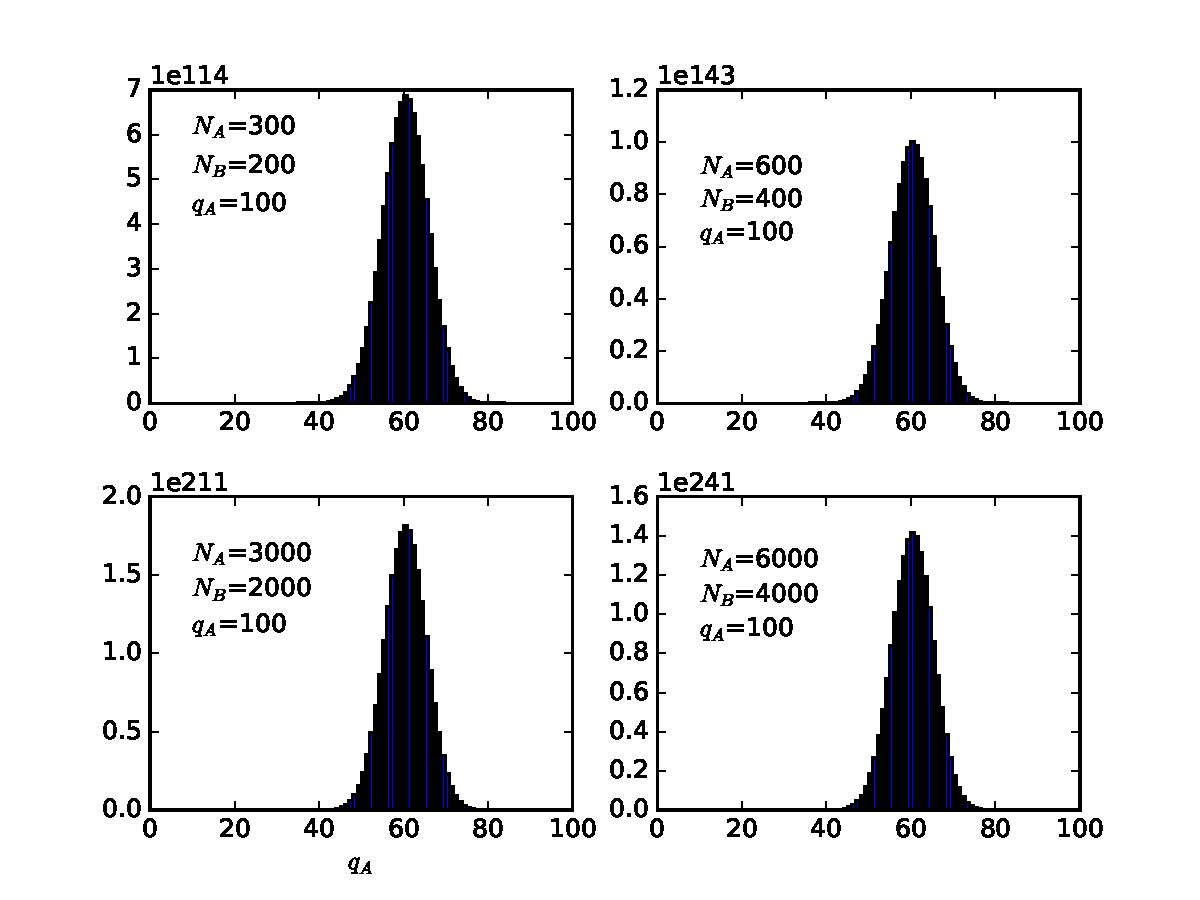
\includegraphics[width=12cm]{Einstein}
\caption{$\Omega$ as a function of $N$ in two interacting Einstein solids. }
\end{figure}
\item Write a code to calculate the probability of $\Omega(q_A)$, when $N_A$=[300, 3000], $N_B$=[200, 2000],
for $q$=[100, 1000], plot them and try to explain the differences. (hint: 2 plots)

\begin{figure}[h]
\centering
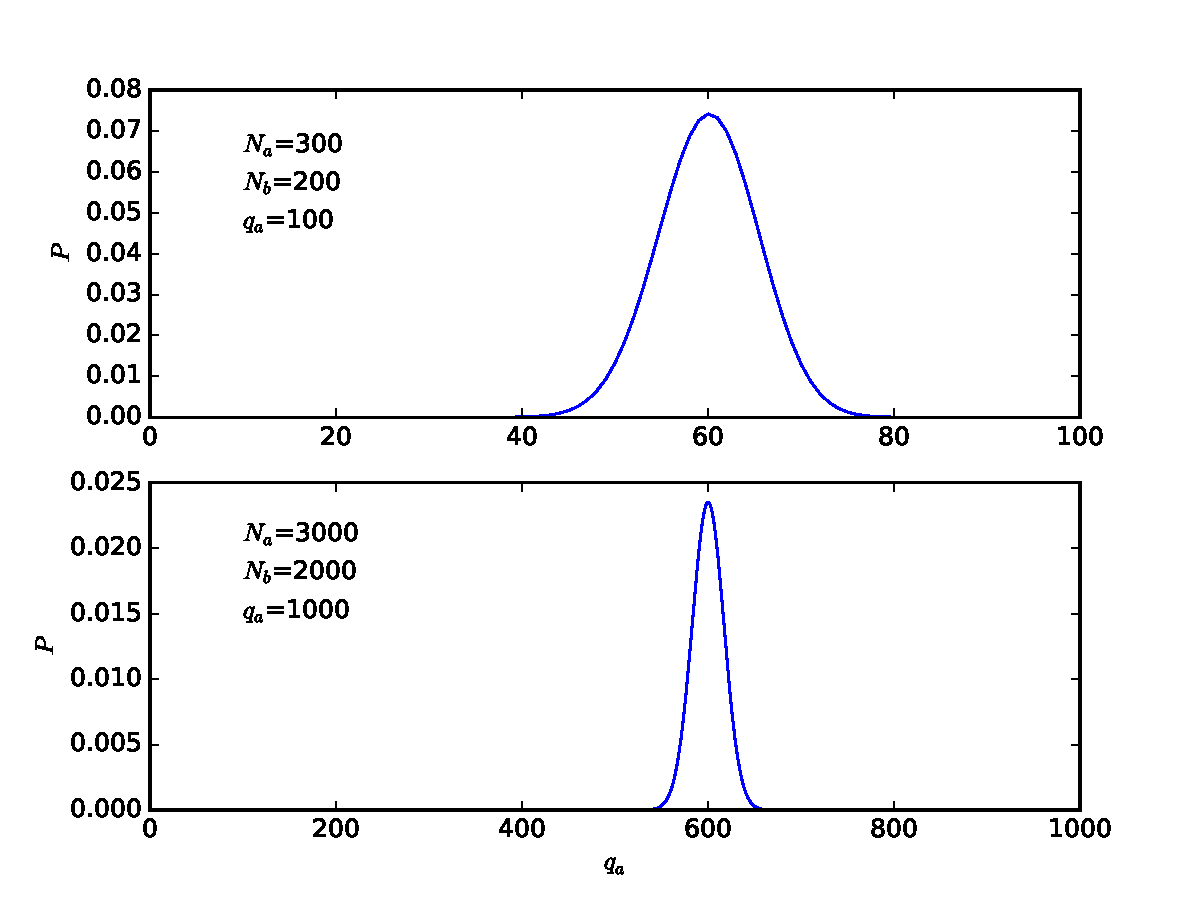
\includegraphics[width=10cm]{Einstein2}
\caption{Probabilty distribution of $\Omega(N)$ in two interacting Einstein solids for different $q$ values. }
\end{figure}

\item Write a code to show the comparison of Stirling's approximation in eq.\ref{s1} and \ref{s2}
\begin{figure}[h]
\centering
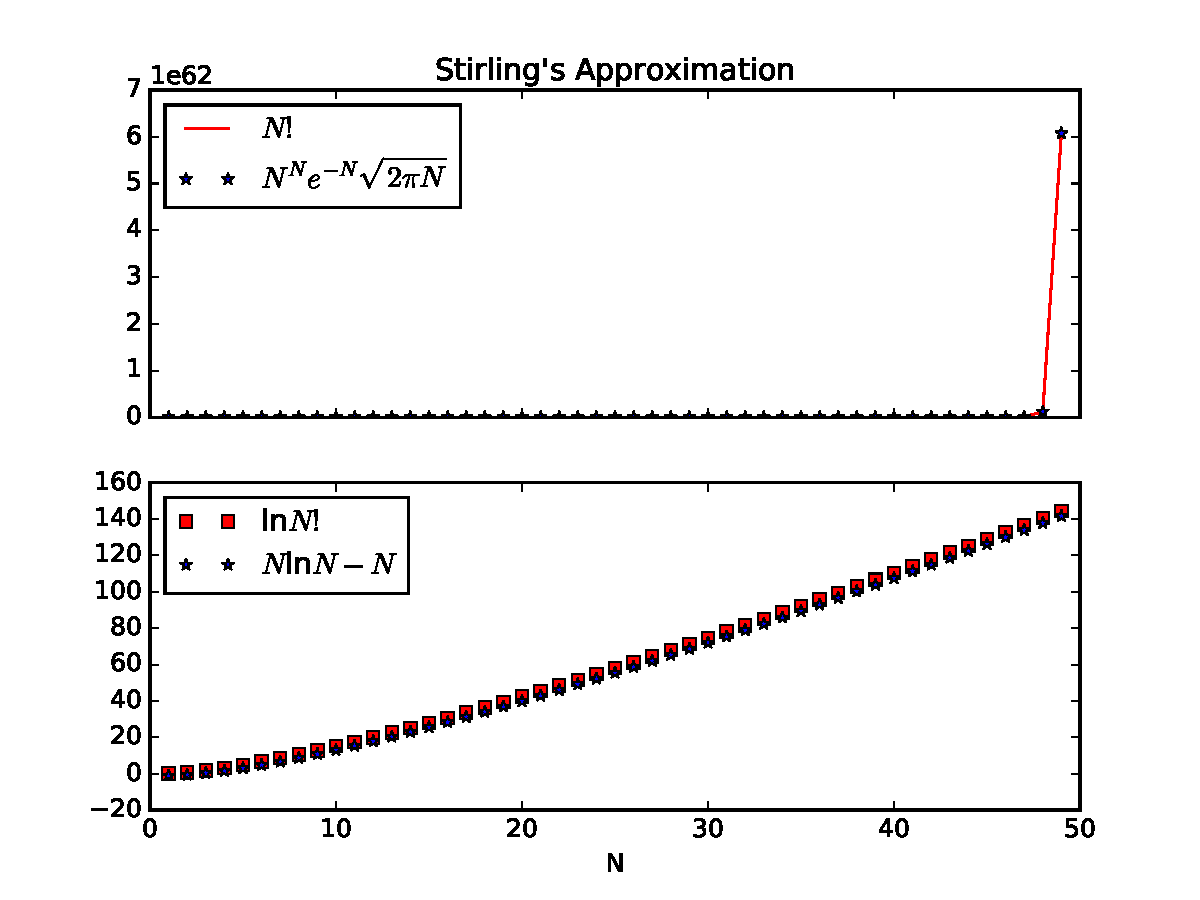
\includegraphics[width=8cm]{Stirling}
\caption{The accuracy of Stirling approximation. }
\end{figure}

\item The Gamma function is defined as 
\begin{equation} \Gamma(n+1) = \int ^\infty _0 x^n e^{-x} dx, \end{equation}
write a code to show the comparsion of $\Gamma(n+1)$, $n$!, and $\sqrt{2\pi n}(n/e)^n$ in the range of [0,3.6]
\begin{figure}[h]
\centering
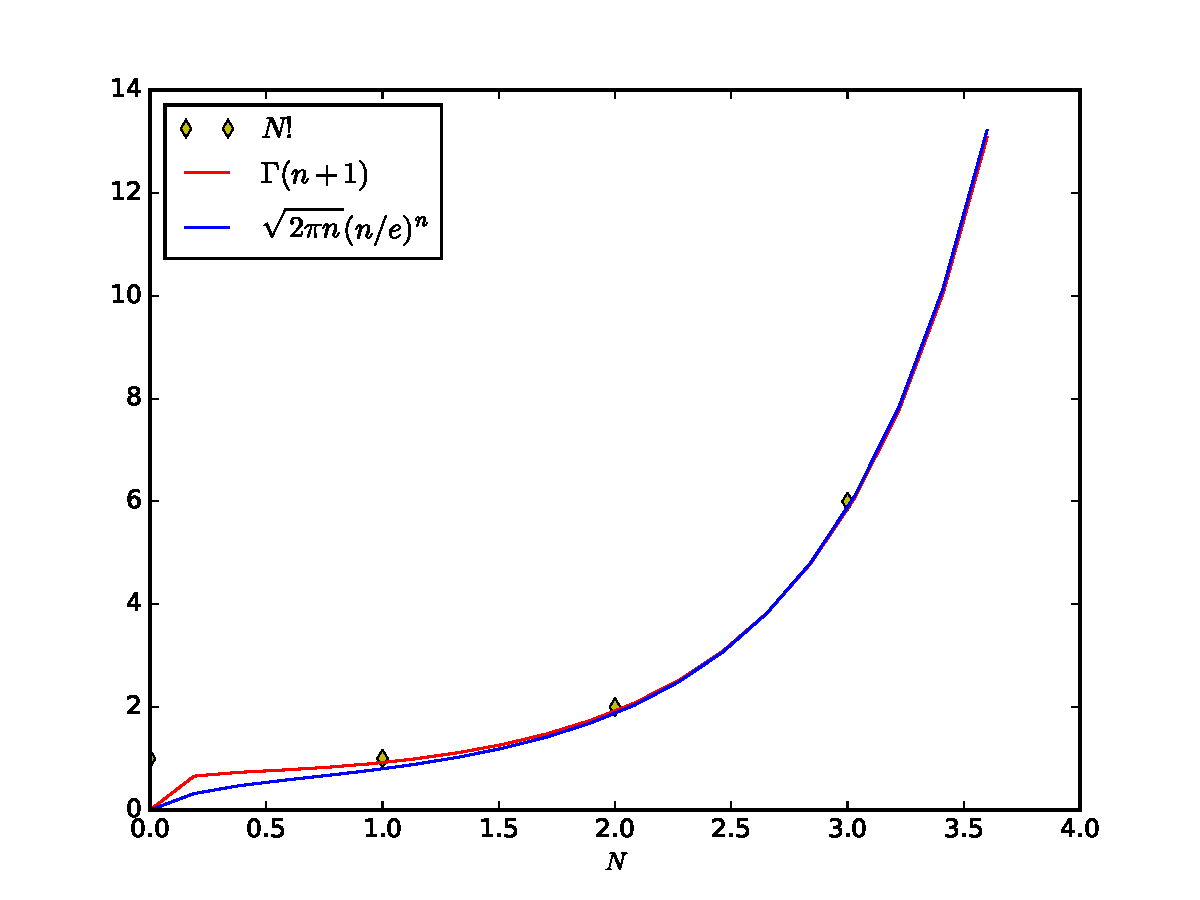
\includegraphics[width=6cm]{Stirling2}
\caption{Comparison between the Gamma function and Stirling approximation. }
\end{figure}


\end{enumerate}
\end{document}
